Tässä kappaleessa käsitellään useamman vuoden käytössä ollutta ratkaisua Drinkkirobotin juomien kaatamiseen.  \todo{Metateksti hyödyllinen?} Ratkaisussa robotin kaadolle on yksittäinen job, joka on esitetty alla.

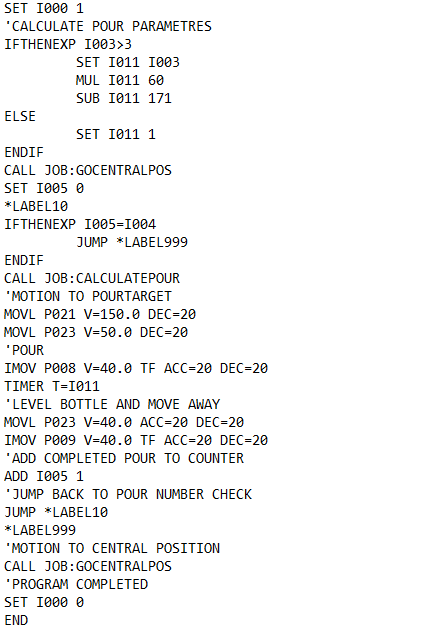
\includegraphics{img/POURDRINKS.png}

Kiinnostavaa jobissa on ensimmäinen if-else-haara, joka käsittelee kaadossa käytetylle ajastimelle annetun arvon laskentaa.

Haluttu kaadon määrä senttilitroina on asetettu muuttujaan I003. POURDRINKS jobi laskee alussa ajan, jonka mukaan robotti kaataa juomaa. Kuten kuvasta nähdään, kaadon aika sekunteina saadaan kaavalla
\[t = 60 \cdot V - 171, \]
jossa V on muuttuja I003, eli haluttu tilavuus senttilitroina. Kyseessä on lineaarinen yhtälö, jossa kulmakerroin 60 ja vakiotermi -171 ovat määritetty kokeellisesti kaatamalla eri määriä juomia.

Jobi toimii siis pääpiirteittäin siten, että robotti liikkuu kohteena olevan mukin kohdalle, kallistaa pulloa ja kun pullo on kallistunut kaatoasentoon, niin käynnistyy ajastin, jonka kesto on määritelty muuttujaan I011.

Ensimmäisen if-elsen tehtävä on myös tarkastaa onko haluttu kaatomäärä alle kolme senttilitraa. Tätä pienemmillä määrillä yllä kuvattu lineaarinen funktio antaisi negatiivisen ajan. Niinpä kaikilla määrillä, jotka ovat alle kolme senttilitraa, kaatoajaksi on määritelty yksi sekunti.
